\documentclass[ngerman,aspectratio=169,10pt]{beamer}

\usetheme[progressbar=frametitle]{metropolis}
\usepackage{appendixnumberbeamer}

\graphicspath{{../graphics/}{.}}

\usepackage{booktabs}
\usepackage{xspace}
\usepackage{amsmath}
\usepackage{amssymb}
\usepackage{amsthm}
\usepackage{xfrac}

\title{External Mergesort}
% \subtitle{}
\date{16. November 2020}
\author{Finn Stutzenstein, Levin Nemesch, Joshua Sangmeister}
\institute{Algorithm Engineering - Übung 1}
\titlegraphic{
    \hfill
\includegraphics[height=1.5cm]{unilogo.pdf}\\
    \hspace*{8.3cm} \textsc{AG Theoretische Informatik}
}

\begin{document}
	
\maketitle

%\section{Überblick}
\begin{frame}{Überblick}
\begin{itemize}
    \item Parameter
    \begin{itemize}
        \item M: Größe des internen Speichers in Byte
        \item B: Blockgröße in Byte
        \item Q: Elementgröße in Bit
    \end{itemize}
    \item Achtung: Effektive Anzahl der Elemente pro Block und im Speicher ist unterschiedlich bei variierendem Q.
    \item L1, L2, L3 Caches:\\[10pt]
    \begin{tabular}{ |l|c|c|c|c| } 
    \hline
     & CPU & L1 & L2 & L3 \\
     \hline
     Finn & i5-3360M & 64 KiB & 512 KiB & 3 MiB \\
     Levin & i5-5200U & 64 KiB & 512 KiB & 3 MiB \\
     Joshua & i5-8265U & 128 KiB & 1 MiB & 6 MiB \\
    \hline
    \end{tabular} \\[10pt]
    \item Code: https://github.com/jsangmeister/AE/tree/master/ue/ue1
\end{itemize}
\end{frame}

%\section{Ergebnisse}
\begin{frame}{Blockgröße}
Sehr große Blöcke (128k und 512k) erhöhen Laufzeit.
\begin{figure}[H]
    \centering
    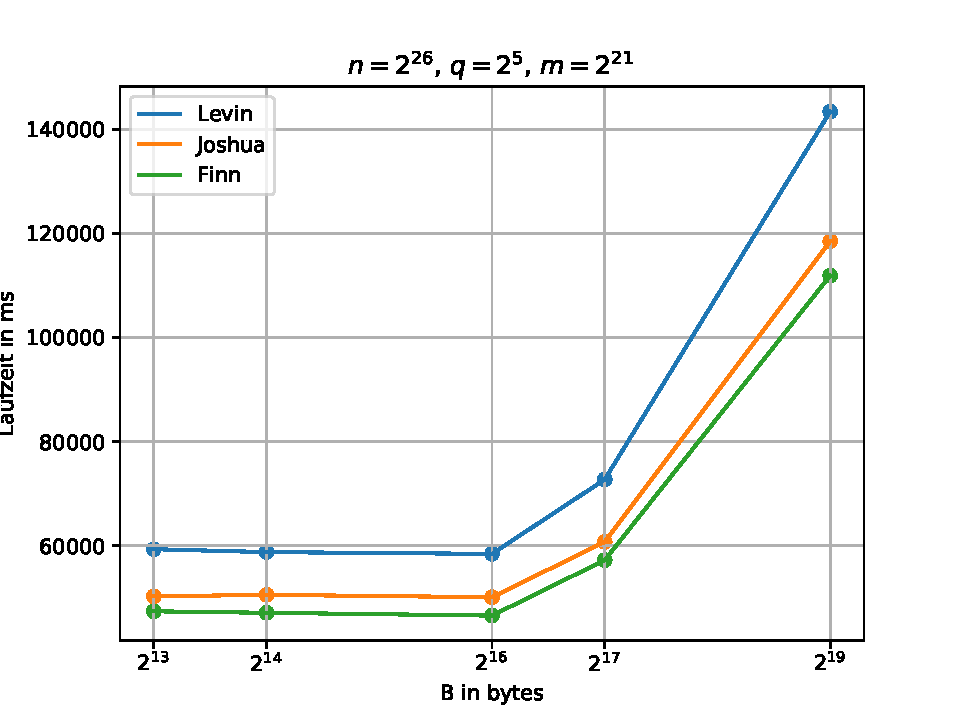
\includegraphics[width=0.65\textwidth]{b__n_67108864_q_32_m_2097152.pdf}
    \label{fig:Figure2}
\end{figure}
\end{frame}

\begin{frame}{Blockgröße}
Sehr große Blöcke (128k und 512k) erhöhen Laufzeit.
\begin{figure}[H]
    \centering
    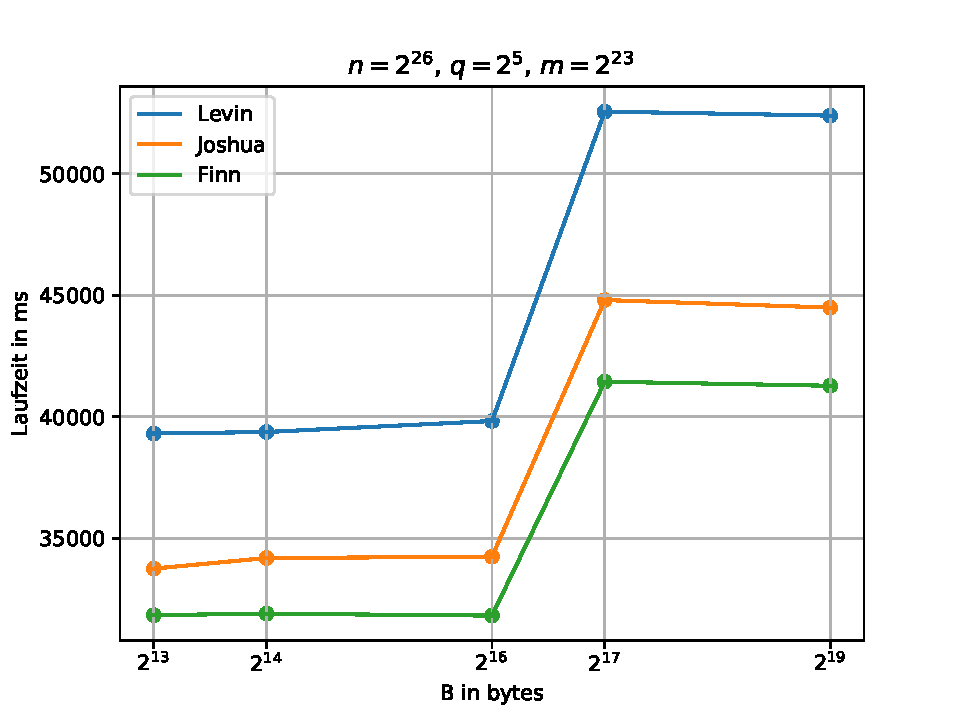
\includegraphics[width=0.65\textwidth]{Figure_1.pdf}
    \label{fig:Figure1}
\end{figure}
\end{frame}

\begin{frame}{Blockgröße}
Sehr große Blöcke (128k und 512k) erhöhen Laufzeit. Warum?
\begin{itemize}
    \item Tatsächliches B der Systeme wird überschritten
    \item Größe der schnellen Caches (L1) wird überschritten
\end{itemize}
\end{frame}

\begin{frame}{Memory}
Bei mehr internem Speicher wie erwartet schneller
\begin{figure}[H]
    \centering
    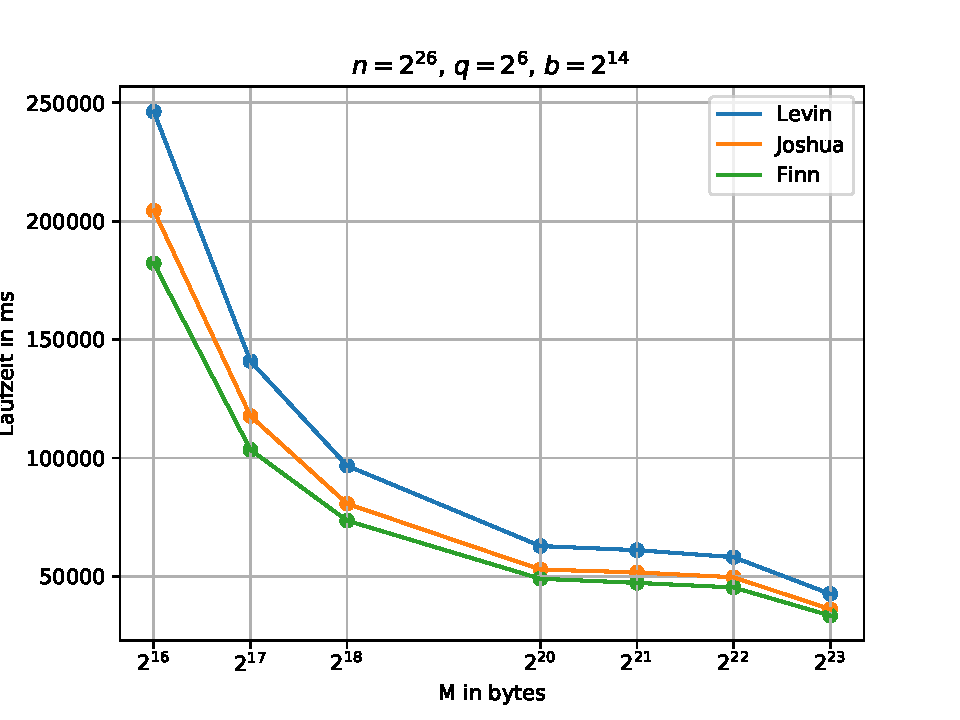
\includegraphics[width=0.65\textwidth]{m__n_67108864_q_64_b_16384.pdf}
    \label{fig:f1}
\end{figure}
\end{frame}

\begin{frame}{Q}
Größere Elemente bedeutet für großes n weniger Elemente pro Block und im Speicher, d.h. die effektive Block- und Speichergröße sinkt.
\vspace{-10pt}
\begin{figure}[H]
    \centering
    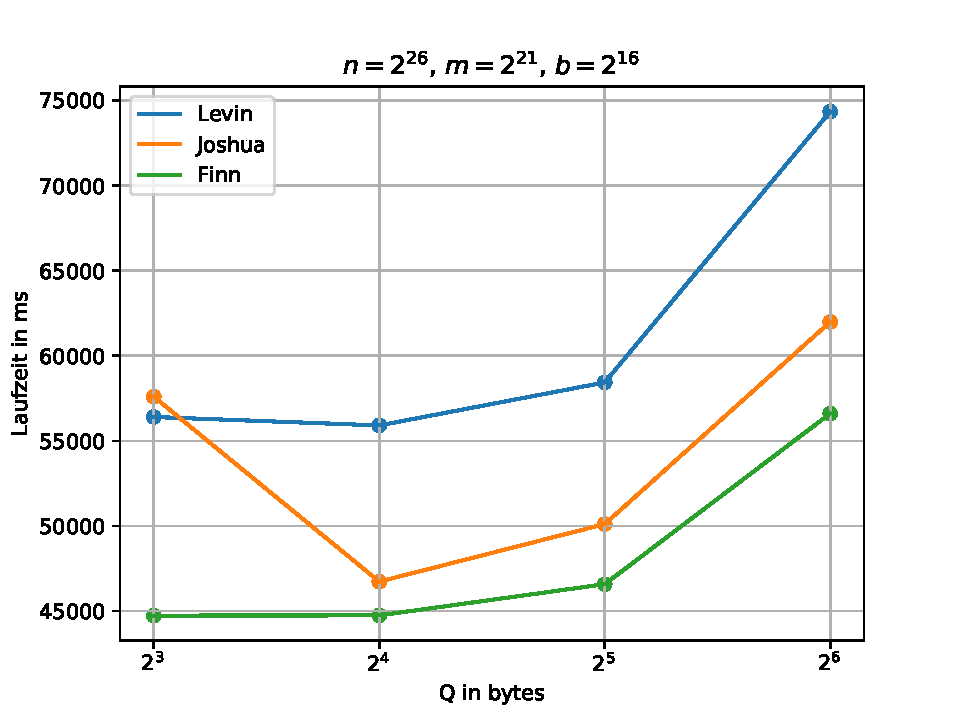
\includegraphics[width=0.65\textwidth]{q__n_67108864_m_2097152_b_65536.pdf}
    \label{fig:f3}
\end{figure}
\end{frame}

\begin{frame}{Q}
Joshua hat bei $n=2^{22}$, $Q=8$ und $Q=16$ durchweg erhöhte Laufzeiten. Die Ursache ist nicht klar.
\vspace{-10pt}
\begin{figure}[H]
    \centering
    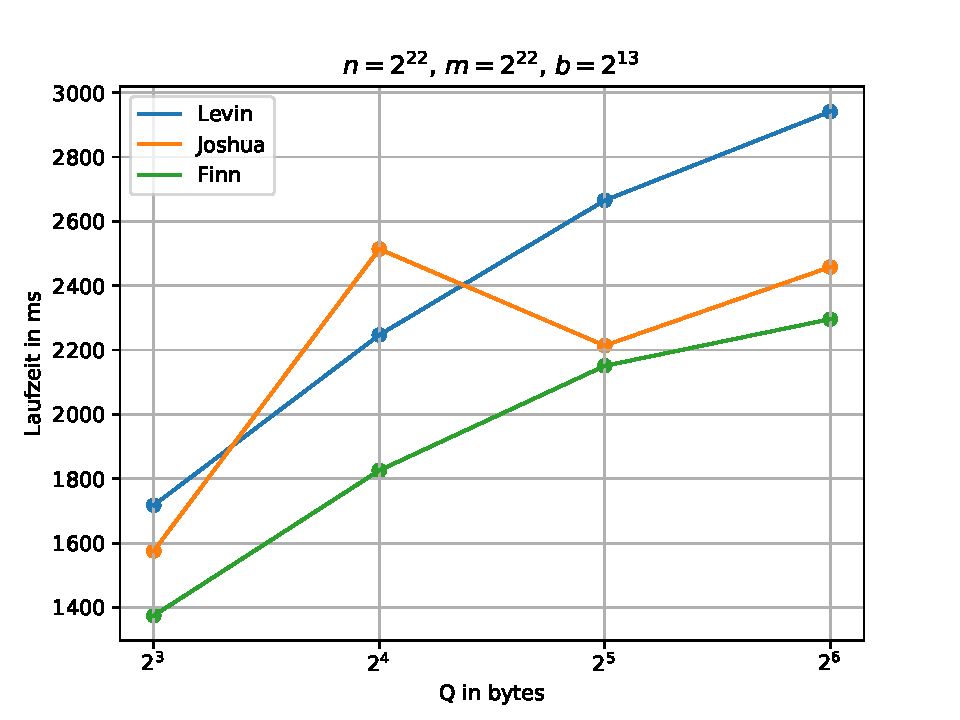
\includegraphics[width=0.65\textwidth]{q__n_4194304_m_4194304_b_8192.pdf}
    \label{fig:f4}
\end{figure}
\end{frame}

\begin{frame}{Q}
Ein ähnlicher Effekt zeigt sich bei $n=2^{23}$ für uns alle
\begin{figure}[H]
    \centering
    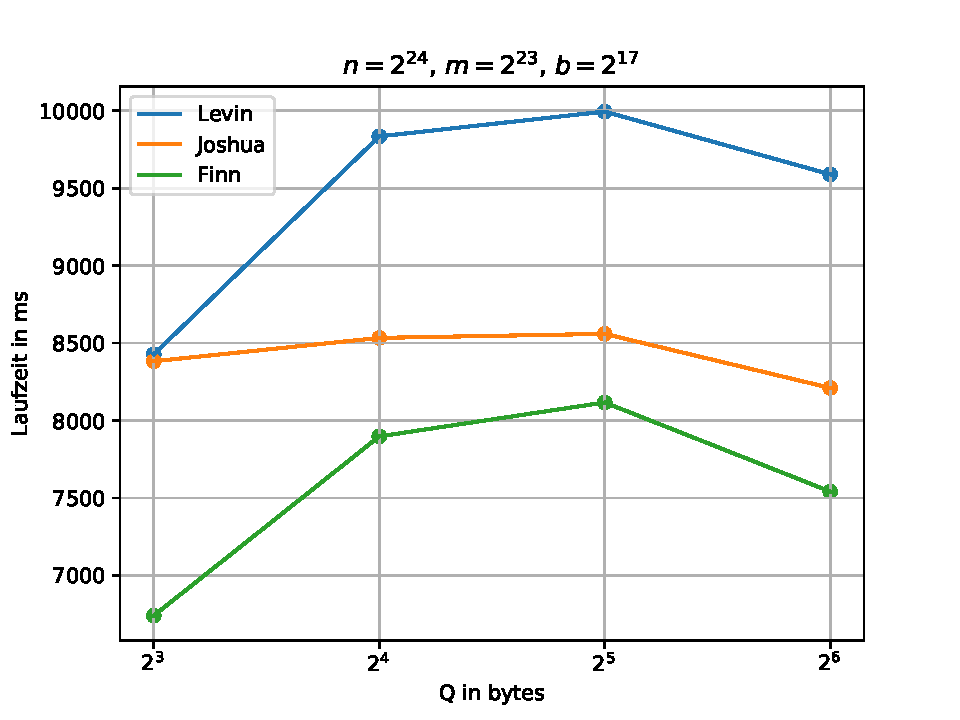
\includegraphics[width=0.65\textwidth]{q__n_16777216_m_8388608_b_131072.pdf}
    \label{fig:f5}
\end{figure}
\end{frame}

\begin{frame}{N}
Wachsende Anzahl Elemente führt zu linearem Wachstum\\
TODO an Joshua: Mit linearer X-Achse plotten.
\begin{figure}[H]
    \centering
    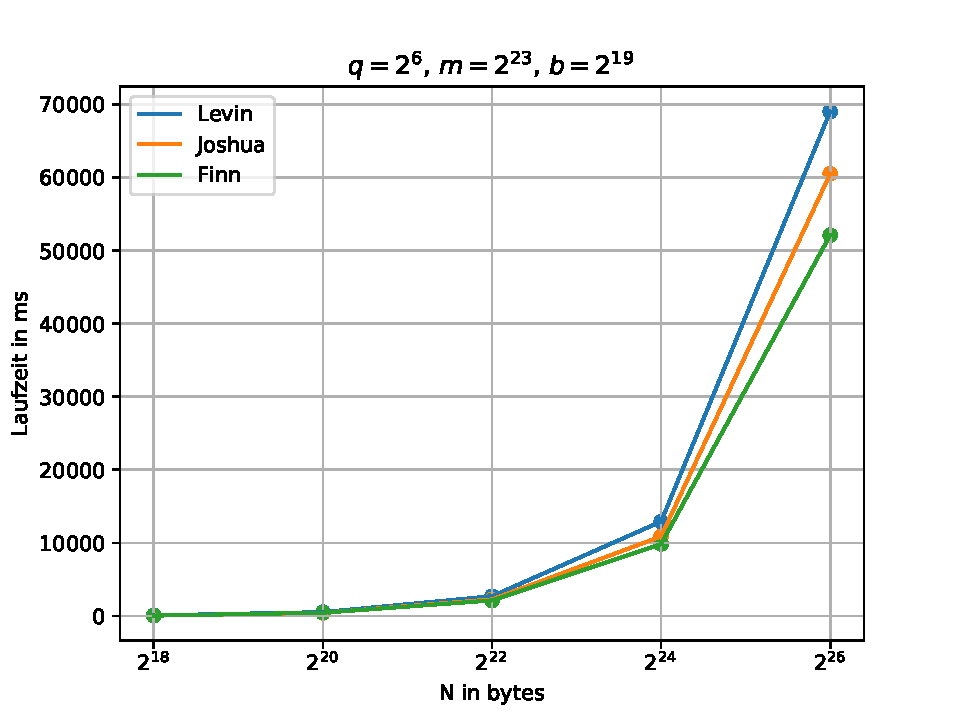
\includegraphics[width=0.65\textwidth]{n__q_64_m_8388608_b_524288.pdf}
    \label{fig:f2}
\end{figure}
\end{frame}

\begin{frame}{N}
TODO an Joshua: Suche dir eine fixe Person, fixes b (eher klein) und plotte alle n gegen zeit für alle m's

TODO an Joshua: Selbe fixe Person, fixes m (eher groß) und plotte alle n gegen zeit für alle b's
\end{frame}

\begin{frame}{N}
TODO an Joshua: Laufzeit pro Element für beide Szenarien oben.
\end{frame}

\begin{frame}{Fazit}
\begin{itemize}
    \item Für wachsendes n steigt die Laufzeit fast linear, der starke Logarithmus in der I/O-Komplexität
\end{itemize}
\end{frame}

\end{document}
